% Figure source. `npm run notes -- build stat497` compiles it to the PDF the
% notes include and to white-noise.svg for the web page. One simulated
% realization of white noise: 200 draws from N(0, 1), generated once with a
% fixed seed (497), so the figure never changes between builds.
\documentclass[tikz,border=4pt]{standalone}
\usepackage{libertinus}
\usepackage{libertinust1math}
\usepackage{pgfplots}
\pgfplotsset{compat=1.18}
\definecolor{accent}{HTML}{1D4E89}
\definecolor{caution}{HTML}{9B2C2C}
\definecolor{quiet}{HTML}{6B7280}
\definecolor{hair}{HTML}{D5D9DF}

\begin{document}
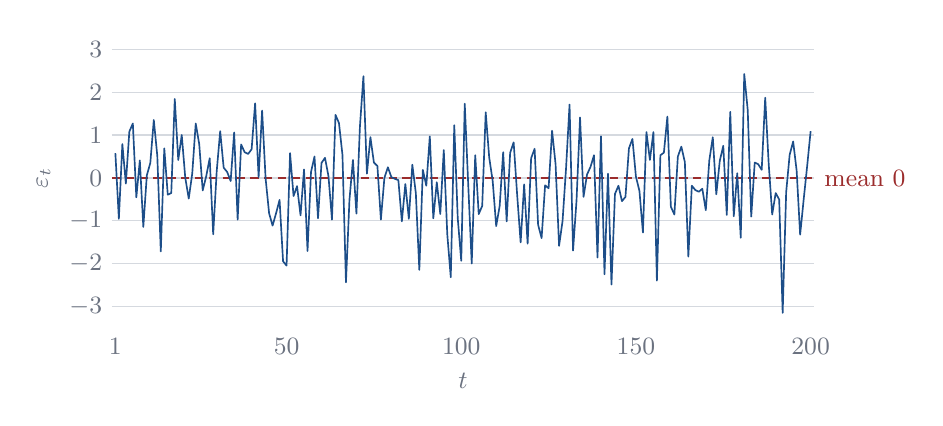
\begin{tikzpicture}
  \begin{axis}[
      width=10.5cm, height=5.4cm,
      xmin=0, xmax=201, ymin=-3.5, ymax=3.5,
      xtick={1,50,100,150,200}, ytick={-3,...,3},
      xlabel={$t$}, ylabel={$\varepsilon_t$},
      label style={font=\small, text=quiet},
      axis line style={draw=none}, tick style={draw=none},
      ymajorgrids, grid style={hair, line width=.4pt},
      tick label style={font=\small, text=quiet},
      clip=false,
    ]
    % The theoretical mean.
    \draw[caution, densely dashed, line width=.8pt] (axis cs:0,0) -- (axis cs:201,0)
      node[right, font=\small, text=caution] {mean $0$};
    \addplot[accent, line width=.6pt, line join=round] coordinates {
      (1,0.58) (2,-0.95) (3,0.79) (4,-0.13) (5,1.08) (6,1.27) (7,-0.45) (8,0.41) (9,-1.14) (10,0.06)
      (11,0.35) (12,1.35) (13,0.52) (14,-1.71) (15,0.69) (16,-0.39) (17,-0.35) (18,1.84) (19,0.42) (20,1.00)
      (21,0.01) (22,-0.48) (23,0.10) (24,1.27) (25,0.79) (26,-0.29) (27,0.04) (28,0.46) (29,-1.31) (30,0.15)
      (31,1.09) (32,0.24) (33,0.14) (34,-0.07) (35,1.06) (36,-0.97) (37,0.78) (38,0.60) (39,0.56) (40,0.67)
      (41,1.74) (42,0.02) (43,1.57) (44,-0.01) (45,-0.82) (46,-1.11) (47,-0.82) (48,-0.51) (49,-1.94) (50,-2.04)
      (51,0.58) (52,-0.42) (53,-0.19) (54,-0.87) (55,0.20) (56,-1.70) (57,0.14) (58,0.50) (59,-0.94) (60,0.35)
      (61,0.47) (62,0.04) (63,-0.97) (64,1.47) (65,1.28) (66,0.54) (67,-2.43) (68,-0.51) (69,0.42) (70,-0.83)
      (71,1.20) (72,2.37) (73,0.10) (74,0.95) (75,0.36) (76,0.28) (77,-0.97) (78,0.00) (79,0.25) (80,0.02)
      (81,-0.02) (82,-0.05) (83,-1.01) (84,-0.14) (85,-0.95) (86,0.31) (87,-0.35) (88,-2.14) (89,0.19) (90,-0.18)
      (91,0.97) (92,-0.94) (93,-0.10) (94,-0.84) (95,0.65) (96,-1.31) (97,-2.31) (98,1.23) (99,-0.94) (100,-1.93)
      (101,1.73) (102,-0.16) (103,-1.99) (104,0.53) (105,-0.84) (106,-0.65) (107,1.53) (108,0.48) (109,-0.07) (110,-1.12)
      (111,-0.65) (112,0.60) (113,-1.01) (114,0.59) (115,0.83) (116,-0.39) (117,-1.50) (118,-0.15) (119,-1.53) (120,0.46)
      (121,0.68) (122,-1.09) (123,-1.40) (124,-0.17) (125,-0.24) (126,1.10) (127,0.32) (128,-1.58) (129,-1.00) (130,0.23)
      (131,1.71) (132,-1.69) (133,-0.52) (134,1.41) (135,-0.44) (136,0.08) (137,0.26) (138,0.53) (139,-1.85) (140,0.97)
      (141,-2.24) (142,0.10) (143,-2.48) (144,-0.37) (145,-0.18) (146,-0.54) (147,-0.44) (148,0.69) (149,0.91) (150,0.03)
      (151,-0.30) (152,-1.27) (153,1.07) (154,0.42) (155,1.07) (156,-2.39) (157,0.53) (158,0.59) (159,1.43) (160,-0.67)
      (161,-0.85) (162,0.50) (163,0.73) (164,0.37) (165,-1.83) (166,-0.18) (167,-0.28) (168,-0.32) (169,-0.25) (170,-0.75)
      (171,0.41) (172,0.95) (173,-0.38) (174,0.40) (175,0.75) (176,-0.86) (177,1.54) (178,-0.89) (179,0.11) (180,-1.39)
      (181,2.42) (182,1.58) (183,-0.90) (184,0.36) (185,0.32) (186,0.19) (187,1.87) (188,0.33) (189,-0.85) (190,-0.35)
      (191,-0.50) (192,-3.14) (193,-0.33) (194,0.54) (195,0.85) (196,0.17) (197,-1.32) (198,-0.51) (199,0.27) (200,1.09)
    };
  \end{axis}
\end{tikzpicture}
\end{document}
